\errorcontextlines=200
\documentclass[twoside,openright]{scrreprt}

\usepackage[msc]{tugrazthesis}
\usepackage{filecontents}  % for the integrated bibliography file (backwards compatibility)
\usepackage[backend=bibtex,style=alphabetic]{biblatex}  % to generate the bibliography
\usepackage{tikz}
\usetikzlibrary{arrows.meta}
\usetikzlibrary{tikzmark,calc}
\addbibresource{\jobname-example.bib}  % name of the bib-file


\begin{document}

%--- INFORMATION FOR TITLEPAGE -------------------------------------------------

% Your name including previous academic degrees (optional argument sets a different \author{}):
\thesisauthor[Firstname Lastname]{Christian Pasero, BSc}

% Title of your thesis (optional argument sets a different \title{}):
\thesistitle[Short Thesis Title]{Computation of Clustered\\Argumentation Frameworks via\\Boolean Satisfiability}

% Date of completion (optional argument sets a different \date{})
\thesisdate[ ]{\today}

% Supervisor headline (select male/female/plural version)
\supervisortitle{\germanenglish{Betreuer}{Supervisor}}

% Supervisor info
\supervisor{
Johannes P. Wallner, Ass.Prof. Dipl.-Ing. Dr.techn. BSc.\\
Institute of Software Technology
}


%\academicdegree{Diplom-Ingenieur/Diplom-Ingenieurin}
\academicdegree{Master of Science}

% Name of your degree programme according to your curriculum (only for msc/diplom
\curriculum{Computer Science}
%--- FRONT MATTER --------------------------------------------------------------

% Insert title page and affidavit

\printthesistitle

% Other front matter you may want to include

\chapter*{Abstract}

English abstract of your thesis

\chapter*{Kurzfassung}

Deutsche Kurzfassung der Abschlussarbeit

% You will typically include *both a German and an English abstract*.
% The rest of the document will be either in German or in English.

\cleardoublepage

\chapter*{\germanenglish{Danksagung}{Acknowledgements}}

\germanenglish{Danke an alle, die beigetragen haben.}{Thanks to everyone who made this thesis possible}
% ...

\cleardoublepage

\tableofcontents

\listoffigures

\listoftables

\chapter*{\germanenglish{Abk\"{u}rzungs- und Symbolverzeichnis}
{List of Acronyms and Symbols}}

% ...



%--- MAIN CONTENT --------------------------------------------------------------

\chapter{Introduction}


\chapter{Theory}

\germanenglish{Eine Referenz auf Abbildung~\ref{fig:dummy}, Tabelle~\ref{tab:dummy}, und ein Buch \cite{Knuth97}.}
{A reference to Figure~\ref{fig:dummy}, Table~\ref{tab:dummy}, and a book \cite{Knuth97}.}

\begin{figure}
	\tikz\draw rectangle (\textwidth,3cm);
	\caption{\germanenglish{Eine Abbildungsunterschrift f\"{u}r das Abbildungsverzeichnis.}
	{A figure caption for the list of figures.}}
	\label{fig:dummy}
\end{figure}

\begin{table}
	\centering
	\begin{tabular}{ll}
		A       & small \\
		example & table \\
	\end{tabular}
	\caption{\germanenglish{Eine Tabellenunterschrift f\"{u}r das Tabellenverzeichnis.}
	{A table caption for the list of tables.}}
	\label{tab:dummy}
\end{table}


% For 45° line -> center + 0.21
% For 22.5° line -> center.x + 0.27 , center.y + 0.11
% Cluster attacks -> cluster.y + 0.21 for top and - 0.21 for bottom
\newcommand{\DrawSelfAttackLeftTopCluster}[2]{% X, Y
\draw[-{To[length=4, width=5]}, line width=0.3mm] (#1, #2) 
.. controls (#1 -0.35, #2 + 0.34) and (#1 - 0.75, #2 - 0.12) .. 
(#1 - 0.13, #2 - 0.12);
}

\newcommand{\DrawAttackDiagonal}[5]{%Direction L.x L.y R.x R.y 
% Direction -> N = Negative slope LR = Left to Right
% Direction -> N = Negative slope RL = Right to Left
% Direction -> P = Positive slope LR = Left to Right
% Direction -> P = Positive slope RL = Right to Left
% Direction -> H = not 45° but Halfed=22.5°
\ifthenelse{\equal{#1}{NLR}}{
\draw[-{To[length=4, width=5]}, line width=0.3mm] (#2 + 0.21,#3 - 0.21) -- (#4 - 0.21 , #5 + 0.21);
}{
\ifthenelse{\equal{#1}{NRL}}{
\draw[-{To[length=4, width=5]}, line width=0.3mm] (#2 - 0.21,#3 + 0.21) -- (#4 + 0.21 , #5 - 0.21);
}{
\ifthenelse{\equal{#1}{PLR}}{
\draw[-{To[length=4, width=5]}, line width=0.3mm] (#2 + 0.21,#3 + 0.21) -- (#4 - 0.21 , #5 - 0.21);
}{
\ifthenelse{\equal{#1}{PRL}}{
\draw[-{To[length=4, width=5]}, line width=0.3mm]  (#2 - 0.21 , #3 - 0.21) -- (#4 + 0.21,#5 + 0.21);
}{}}}}}

\newcommand{\DrawAttackHorizontal}[5]{%Direction L.x L.y R.x R.y 
% R = Right to Left
% L = Left to Right
\ifthenelse{\equal{#1}{R}}{
\draw[-{To[length=4, width=5]}, line width=0.3mm] (#2 + 0.3,#3) -- (#4 - 0.3 , #5);
}{
\ifthenelse{\equal{#1}{L}}{
\draw[-{To[length=4, width=5]}, line width=0.3mm]  (#2 - 0.3,#3) -- (#4 + 0.3 , #5);
}{}}}


\newcommand{\DrawAttackVertical}[5]{%Direction L.x L.y R.x R.y 
% U = Down to Top
% D = Top to Down
% B = Double Attack
\ifthenelse{\equal{#1}{U}}{
\draw[-{To[length=4, width=5]}, line width=0.3mm] (#2,#3 + 0.3) -- (#4, #5 - 0.3);
}{
\ifthenelse{\equal{#1}{D}}{
\draw[-{To[length=4, width=5]}, line width=0.3mm] (#2,#3 - 0.3) -- (#4, #5 + 0.3);
}{
\ifthenelse{\equal{#1}{B}}{
\draw[-{To[length=4, width=5]}, line width=0.3mm] (#2 + 0.08, #3 - 0.3) -- (#4 + 0.08, #5 + 0.3);
\draw[{To[length=4, width=5]}-, line width=0.3mm] (#2 - 0.08, #3 - 0.3) -- (#4 - 0.08, #5 + 0.3);

}{}}}}




\chapter{Examples}
Wtf is going on.
\section{Basic AF}
\subsection{Concrete AF}
\begin{center}
	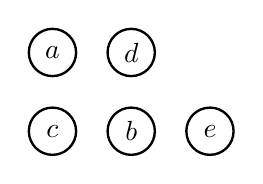
\begin{tikzpicture}
		% Singletons
		\def \ax{0}   \def \ay{0}
		\def \bx{1}   \def \by{-1}
		\def \cx{0}   \def \cy{-1}
		\def \dx{1}   \def \dy{0}
		\def \ex{2}   \def \ey{-1}

		\draw[line width=0.3mm] (\ax, \ay) circle (0.3) node[anchor=center]{$a$};
		\draw[line width=0.3mm] (\bx, \by) circle (0.3) node[anchor=center]{$b$};
		\draw[line width=0.3mm] (\cx, \cy) circle (0.3) node[anchor=center]{$c$};
		\draw[line width=0.3mm] (\dx, \dy) circle (0.3) node[anchor=center]{$d$};
		\draw[line width=0.3mm] (\ex, \ey) circle (0.3) node[anchor=center]{$e$};
		% Attacks
		% a - c
		% c - a
		\DrawAttackVertical{B}  {\ax}{\ay}{\cx}{\cy}
		% a - b
		\DrawAttackDiagonal{NLR}{\ax}{\ay}{\bx}{\by}
		% a - d
		\DrawAttackHorizontal{R}{\ax}{\ay}{\dx}{\dy}
		% d - e
		\DrawAttackDiagonal{NLR}{\dx}{\dy}{\ex}{\ey}
		% e - b
		\DrawAttackHorizontal{L}{\ex}{\ey}{\bx}{\by}
	\end{tikzpicture}
\end{center}
Stable Sets: $\{\}$, $\{a, e\}$, $\{b, c, d\}$


\subsection{Abstract AF}
\begin{center}
	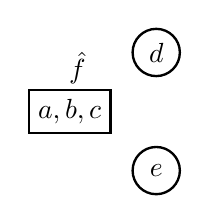
\begin{tikzpicture}
		\def \dx{1.1} \def \dy{0} 
		\def \ex{1.1} \def \ey{-1.5} 
		\def \fx{0}   \def \fy{-0.75}
		% Cluster
		\node[rectangle, draw, line width=0.3mm] at (\fx, \fy) {$a,b,c$};
		\node at (\fx + 0.1, \fy + 0.55) {$\hat{f}$};
		% Singletons
		\draw[line width=0.3mm] (\dx,\dy) circle (0.3) node[anchor=center]{$d$};
		\draw[line width=0.3mm] (\ex,\ey) circle (0.3) node[anchor=center]{$e$};
		% Attacks
		% f - d
		\DrawAttackDiagonal{PLR}{\fx + 0.35}{\fy}{\dx}{\dy}
		% d - e
		\DrawAttackVertical{D}{\dx}{\dy}{\ex}{\ey}
		% e - f
		\DrawAttackDiagonal{NRL}{\ex}{\ey}{\fx + 0.35}{\fy}
		% f - f SELFATTACK
		\DrawSelfAttackLeftTopCluster{-0.45}{-0.44}
	\end{tikzpicture}
\end{center}
Stable Sets: $\{\}$, $\{\hat{f}, e\}$, $\{\hat{f}, d\}$

concrete with main abstract $\rightarrow$ \texttt{FAITHFUL}



\subsection{Abstract AF with Concretized Argument b}
\begin{center}
	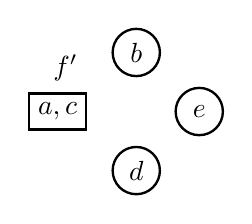
\begin{tikzpicture}
		\def \bx{1} \def \by{0}
		\def \dx{1} \def \dy{-1.5}
		\def \ex{1.8} \def \ey{-0.75}
		\def \fx{0} \def \fy{-0.75}
		% Cluster
		\node[rectangle, draw, line width=0.3mm] at (\fx, \fy) {$a,c$};
		\node at (0.1, -0.2) {$f'$};
		% Singletons
		\draw[line width=0.3mm] (\bx,\by)  circle (0.3) node[anchor=center]{$b$};
		\draw[line width=0.3mm] (\dx,\dy)  circle (0.3) node[anchor=center]{$d$};
		\draw[line width=0.3mm] (\ex,\ey)  circle (0.3) node[anchor=center]{$e$};
		% Attacks
		% f - f SELFATTACK
		\DrawSelfAttackLeftTopCluster{-0.28}{-0.48}
		% f - b
		\DrawAttackDiagonal{PLR}{\fx + 0.2}{\fy}{\bx}{\by}
		% e - b
		\DrawAttackDiagonal{NRL}{\ex}{\ey}{\bx}{\by}
		% d - e
		\DrawAttackDiagonal{PLR}{\dx}{\dy}{\ex}{\ey}
		% f - d
		\DrawAttackDiagonal{NLR}{\fx + 0.2}{\fy}{\dx}{\dy}

	\end{tikzpicture}
\end{center}


%--- BIBLIOGRAPHY --------------------------------------------------------------

% Print bibliography and include it in the table of contents:
\printbibliography[heading=bibintoc]

% An example bibliography file.
%
% This will create a separate file named "thesis-example.bib" and will overwrite
% its content on each compile run.
% If you already have your own bibliography file(s) or prefer to maintain
% thesis.bib separately, update the line "\addbibresource{\jobname.bib}" in the
% preamble and delete the following lines!
\begin{filecontents*}{\jobname-example.bib}

	@book{Knuth97,
	author    = {Donald Ervin Knuth},
	title     = {The Art of Computer Programming, Volume {I}: Fundamental Algorithms, 3rd Edition},
	publisher = {Addison-Wesley},
	year      = {1997},
	}

\end{filecontents*}

\end{document}
